\documentclass[12pt,a4paper]{article}

\usepackage[a4paper,margin=1in]{geometry}
\usepackage{graphicx}
\usepackage{float}
\usepackage{booktabs}
\usepackage{amsmath}
\usepackage{array}
\usepackage{setspace}
\usepackage{caption}
\usepackage{hyperref}
\usepackage{enumitem}
\usepackage{microtype}

\onehalfspacing
\setlength{\parindent}{0pt}
\setlength{\parskip}{6pt}

\title{\textbf{Feature Engineering and Exploratory Analysis of Vehicle Logbook Data}}
\author{Adivhaho Nevondo}
\date{08 September 2026}

\begin{document}

\begin{titlepage}
    \centering
    \vspace*{2cm}
    {\Large\textbf{Feature Engineering and Exploratory Analysis of Vehicle Logbook Data}\par}
    \vspace{1.5cm}
    \vspace{2cm}
    \begin{tabular}{rl}
        \textbf{Student:} & Adivhaho Nevondo \\
        \textbf{Date:} & 08 September 2026 \\
    \end{tabular}
    \vfill
    \vspace{0.5cm}
\end{titlepage}

\tableofcontents
\newpage

\section{Introduction}

The Report focus on \textbf{Section 2 and 3} of the assignment, Feature Engineering and Vehicle Exploration. The are two main aims: first, to transform information stored in semi-structured fields into useful numerical and categorical features(Section 2); and second, to explore patterns in users, application activity, vehicle age, and vehicle popularity(Section 3).

The transformations include extracting currency information, converting monetary fields into numerical values, parsing vehicle and user information from URLs, and converting fuel-consumption measurements from imperial to metric units.

The exploratory analysis subsequently examines unique users by currency, daily application activity, vehicle-age distributions, popular vehicle makes, and the most popular vehicle models. Importantly, currency is used as a \emph{proxy} for country rather than being treated as a direct country identifier. \cite{notebook}

\section{Data Preparation}

The dataset was loaded from the file \texttt{logbook\_assignment1.csv}. During loading, Pandas issued a \texttt{DtypeWarning} for the \texttt{gallons} and \texttt{mpg} columns because these columns contain mixed data types. The subsequent processing therefore explicitly uses numeric coercion where numerical calculations are required. \cite{notebook}

The analysis also establishes a regular-expression pattern containing common currency symbols and abbreviations, including dollar, pound, euro, yen, rupee, rand, Swiss franc, and several ISO-style currency codes. This pattern is subsequently applied to the monetary field \texttt{total\_spent}. \cite{notebook}

\section{Feature Engineering} 

\subsection{Currency extraction}

A new categorical feature, \texttt{\textbf{currency}}, was created by extracting the currency symbol or abbreviation from the existing \texttt{total\_spent} field. The extraction is performed after converting the source field to a string and applying the predefined regular-expression pattern, separating the currency information from the monetary amount and makes the currency available for grouping and exploratory analysis. \cite{notebook}

\subsection{Numerical monetary features}

Two numerical features were created from monetary fields: \texttt{total\_spent\_float} and \texttt{cost\_per\_gallon\_float}. A helper function removes formatting that prevents direct conversion to floating-point values and returns missing values when the source value is missing or cannot be converted.\cite{notebook}

\subsection{Parsing vehicle and user information from URLs}

The Dataset and notebook uses the URL structure containing vehicle information illustrated by an example of the form

\begin{center}
\texttt{https://www.somewebsite.com/suzuki/swift/2015/674857}
\end{center}

The final URL component is extracted as \texttt{user\_id}; the preceding component is parsed for a four-digit \texttt{car\_year}; the preceding components are assigned to \texttt{car\_model} and \texttt{car\_make}, respectively. This transforms information embedded in a URL into explicit dataframe columns. \cite{notebook}

\subsection{Conversion from imperial to metric units}

This sub-section converts fuel and distance measurements into metric units. \textbf{Gallons are converted to litres using the factor 3.78541178}, while \textbf{miles are converted to kilometres using the factor 1.609344}. A fuel-efficiency feature, \texttt{litres\_per\_100km}, is then calculated as

\begin{equation}
    \text{L/100 km} = \frac{\text{litres}}{\text{kilometres}} \times 100.
\end{equation}

These transformations make the measurements more convenient for metric system analysis. \cite{notebook}

\section{Vehicle Exploration Data Analysis}

\subsection{Unique users by currency}

To investigate the geographical distribution of users, group observations by the newly created \texttt{currency} feature and counts the number of distinct user IDs in each group. The analysis explicitly describes currency as a proxy for country.

\begin{figure}[H]
    \centering
    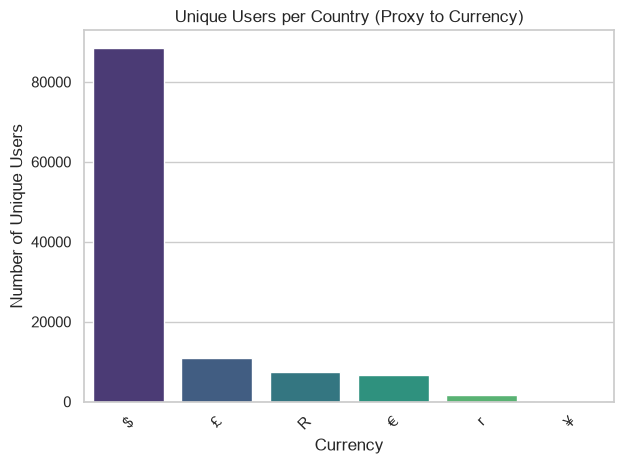
\includegraphics[width=0.82\textwidth]{Unique_users_per_country.png}
    \caption{Number of unique users grouped by currency, used as a proxy for country. The distribution is strongly concentrated in the dollar-denominated group, with substantially smaller user counts in the other currency groups.}
    \label{fig:users-currency}
\end{figure}

Figure~\ref{fig:users-currency} shows a clear imbalance between the currency groups. The dollar group contains by far the largest number of unique users, while the pound, rand, and euro groups form considerably smaller groups. The remaining currency groups contain relatively few users. \cite{notebook}

\subsection{App popularity over time}

Application popularity was examined by converting \texttt{date\_captured} into a date-time representation and counting the number of unique users recorded on each date. The resulting daily counts were plotted as a time series. \cite{notebook}

\begin{figure}[H]
    \centering
    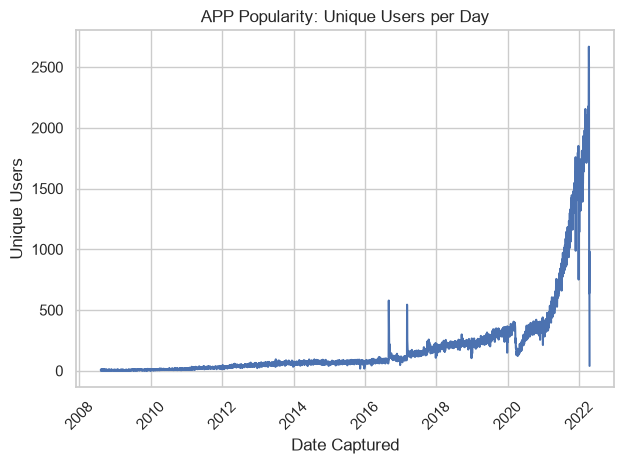
\includegraphics[width=0.88\textwidth]{app_popularity.png}
    \caption{Application popularity measured as the number of unique users per captured date.}
    \label{fig:app-popularity}
\end{figure}

Figure~\ref{fig:app-popularity} indicates relatively low activity during the earlier years, followed by a gradual increase. Activity becomes substantially higher after approximately 2016 and rises particularly sharply toward 2021 and early 2022. The plot also contains several isolated spikes and drops, indicating that daily activity was not uniform throughout the observation period. \cite{notebook}

\subsection{Vehicle age distribution without an age restriction}

Vehicle age was calculated from the difference between the year in which a vehicle was refuelled and the vehicle's extracted model year:

\begin{equation}
    \text{Vehicle Age} = \text{Fueling Year} - \text{Car Year}.
\end{equation}

The compared resulting vehicle-age distributions across currency groups is displayed using boxplots. \cite{notebook}

\begin{figure}[H]
    \centering
    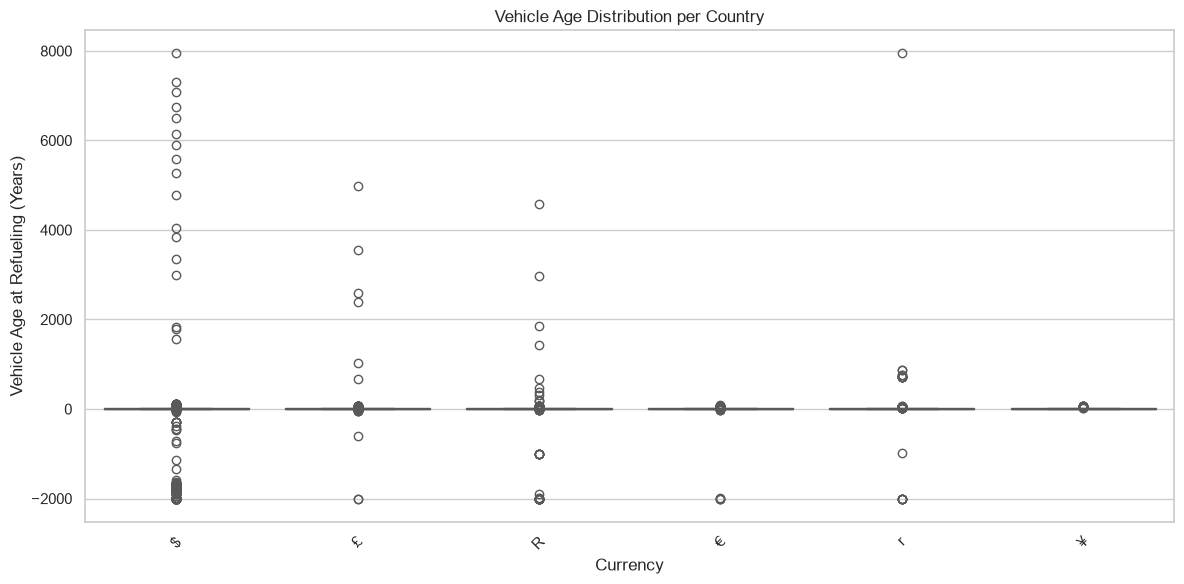
\includegraphics[width=0.96\textwidth]{vehicle_age_distribution_for_all_age.png}
    \caption{Vehicle-age distribution by currency before restricting the calculated ages to a plausible range. The plot contains numerous extreme positive and negative values, demonstrating the presence of implausible calculated ages.}
    \label{fig:vehicle-age-unfiltered}
\end{figure}

The unrestricted plot in Figure~\ref{fig:vehicle-age-unfiltered} demonstrates why a range restriction is useful for interpreting vehicle age. Several observations have extremely large positive ages, while others have negative ages. These values are not meaningful as conventional vehicle ages and can dominate the scale of the visualisation, making the central distributions difficult to inspect.

\subsection{Vehicle age distribution restricted to 50 years}

To produce a more interpretable view, a filtered dataframe was created containing observations satisfying

\begin{equation}
    0 \leq \text{Vehicle Age} \leq 50.
\end{equation}

The resulting distributions are again displayed as boxplots by currency. \cite{notebook}

\begin{figure}[H]
    \centering
    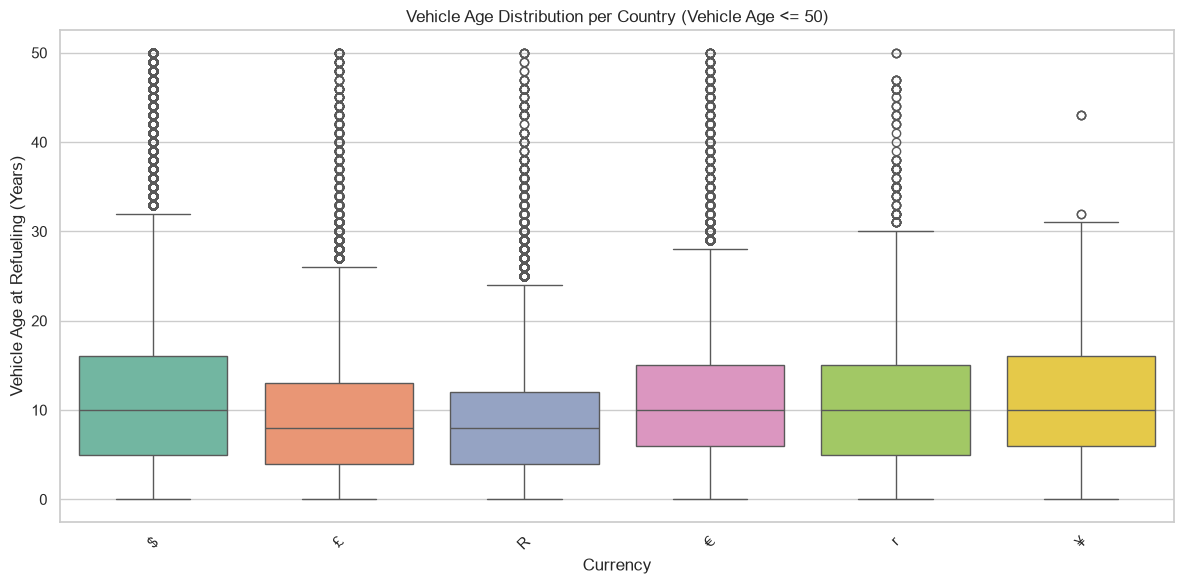
\includegraphics[width=0.96\textwidth]{vehicle_age_distribution_for_realistic_50_years.png}
    \caption{Vehicle-age distribution by currency after restricting vehicle age to the range 0--50 years. The filtered distributions are considerably easier to compare, with central values generally lying in the single- to low-double-digit range.}
    \label{fig:vehicle-age-filtered}
\end{figure}

Figure~\ref{fig:vehicle-age-filtered} provides a substantially clearer comparison. The median vehicle ages for the displayed currency groups are generally around the middle single digits to approximately ten years, while observations extend toward the imposed 50-year upper limit. The filtered representation is therefore more informative for comparing typical vehicle ages than the unrestricted plot.

\subsection{Popular vehicle makes}

Vehicle make popularity was measured using the number of unique users associated with each \texttt{car\_make}. The makes were sorted in descending order and visualised using a horizontal bar chart. \cite{notebook}

\begin{figure}[H]
    \centering
    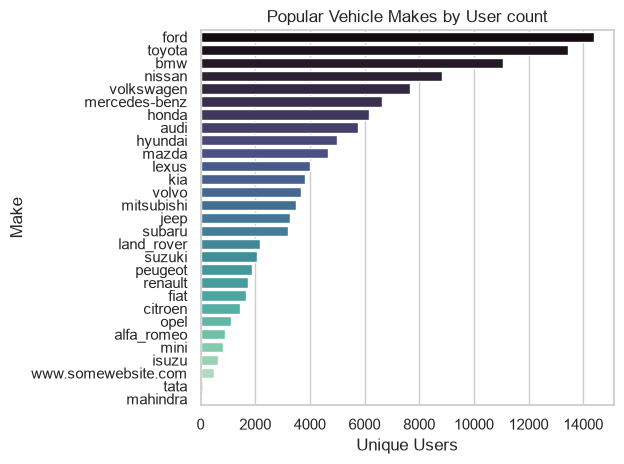
\includegraphics[width=0.88\textwidth]{popular_makes.png}
    \caption{Popular vehicle makes ranked by number of unique users.}
    \label{fig:popular-makes}
\end{figure}

Figure~\ref{fig:popular-makes} shows that the user distribution across makes is highly uneven. A long tail of less frequently represented makes is visible toward the bottom of the ranking.

\subsection{Most popular vehicle models}

A combined \texttt{make\_model} feature was created by concatenating the extracted vehicle make and model. Unique users were then counted for each combined value and the 20 most frequent models were selected. \cite{notebook}

\begin{figure}[H]
    \centering
    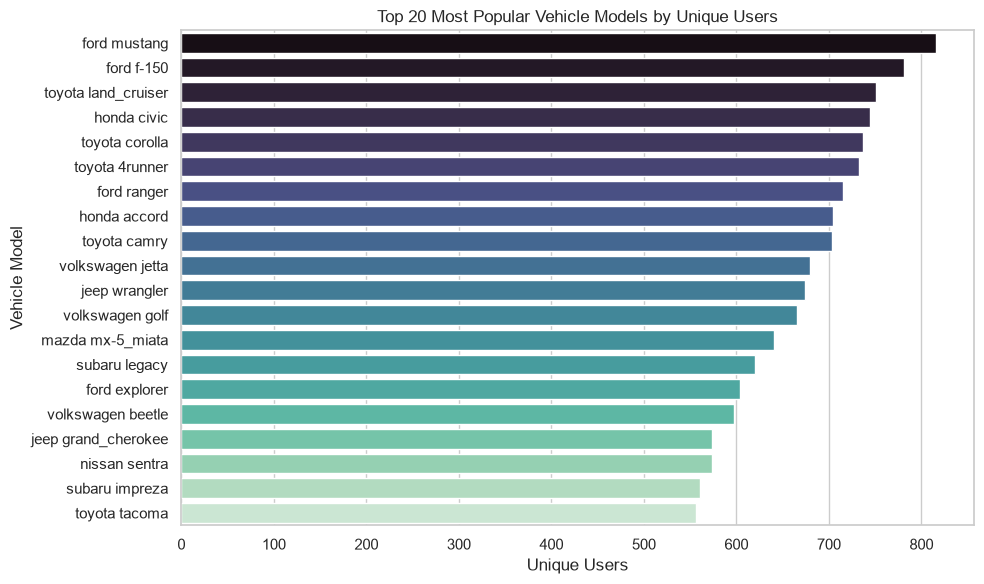
\includegraphics[width=0.96\textwidth]{popular_20_models.png}
    \caption{Top 20 vehicle models ranked by number of unique users.}
    \label{fig:popular-models}
\end{figure}

The model-level ranking in Figure~\ref{fig:popular-models} provides a more detailed view of vehicle popularity than the make-level analysis. The top 20 models all have substantially more users than the remaining models outside the displayed ranking, although the difference between neighbouring entries within the top 20 is comparatively gradual.

\section{Discussion}

The analysis demonstrates how semi-structured vehicle logbook data can be transformed into features suitable for exploratory and subsequent quantitative analysis. In particular, extracting currency, numerical monetary values, vehicle information, and user IDs makes information that was previously embedded in strings directly accessible for grouping and calculation.

The URL parsing step is especially useful because a single field contains several logically distinct attributes. Separating these attributes enables analyses such as vehicle-age calculation and make/model popularity. Similarly, converting gallons and miles into litres and kilometres allows fuel consumption to be expressed in litres per 100 kilometres, a standard metric representation.

Several limitations should nevertheless be considered. The vehicle-age calculation depends on the quality of both the extracted vehicle year and the refuelling date. The unrestricted results demonstrate that the raw calculation contains extreme and negative values. The subsequent 0--50 year filter improves interpretability, but it is an analytical restriction rather than evidence that every excluded observation is necessarily incorrect.

The popularity analysis also relies on unique-user counts. Consequently, the figures describe the number of distinct users associated with each currency, make, or model rather than the number of individual logbook records. This distinction is important when interpreting the results because a single user may contribute multiple observations.


\section{Conclusion}

This report presented the feature engineering and exploratory analysis performed on the vehicle logbook dataset. The main engineered features were currency, numerical monetary values, user ID, vehicle year, vehicle make, vehicle model, litres, kilometres, and litres per 100 kilometres. These transformations converted information from formatted strings and URLs into explicit variables that can be analysed computationally.

The exploratory analysis identified a strong imbalance in unique users across currency groups, increasing application activity over the observed period, and substantial problems with unrestricted vehicle-age calculations. Restricting vehicle age to 0--50 years produced a much more interpretable distribution.


\begin{thebibliography}{9}
\bibitem{notebook}
Jupyter notebook, \textit{feature.ipynb}, ``Feature Engineering and Vehicle Exploration'', September 2026.
\end{thebibliography}

\end{document}
